\section{Beispielformulierungen von Zielen und Problemen}

\subsection{8er Puzzle (Sliding block puzzle)}

\begin{itemize}
    \item Hochgradig kombinatorisches NP-vollst�ndiges Problem. Oft genutzt als Standardtest f�r neue Suchalgorithmen.
\end{itemize}

\begin{figure}[h!]
    \centering
    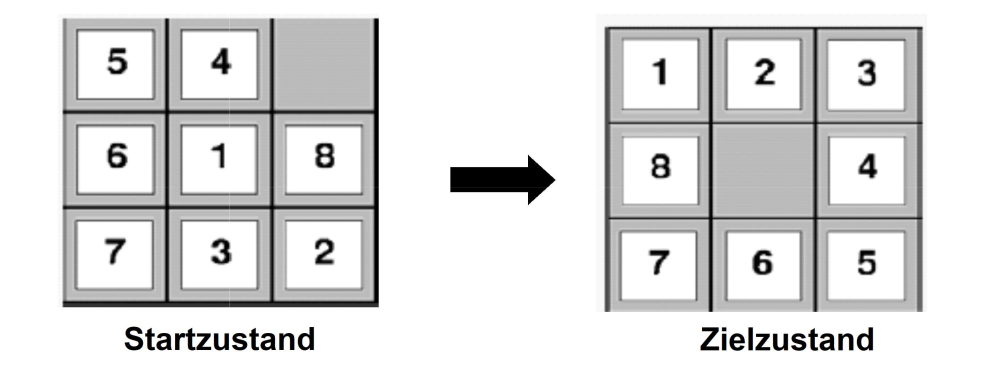
\includegraphics[width=0.8\textwidth]{figures/8er-puzzle.png}
    \caption{8er puzzle Start- und Zielzustand}
    \label{fig:8er-puzzle}
\end{figure}

\begin{itemize}
    \item Zust�nde: Lokalit�t der 8 Fliesen in eine der 9 Fl�chen plus eine freie Kachel
    \item Operatoren: Blank nach Links, Rechts, Auf, Ab 
    \item Ziel-test: Blank-Kachel in der Mitte
    \item Pfadkosten: jeder Schritt kostet eine Einheit
\end{itemize}

\subsection{Staubsauger-Roboter}

Vieles an der Implementierung dieses Roboters muss abstrahiert werden:
\begin{itemize}
    \item World States: Umfassen alle Aspekte der reelen Welt
    \item Problem States: Nur Aspekte der relevant f�r das Problem sind. Die Modellierung von diesen Aspekten erfolgt meist in Form \textbf{symbolisher} Beschreibungen. 
    \item Erstens m�ssen die m�glichen World States als Problem States dargestellt werden:
\end{itemize}

\begin{figure}[h!]
    \centering
    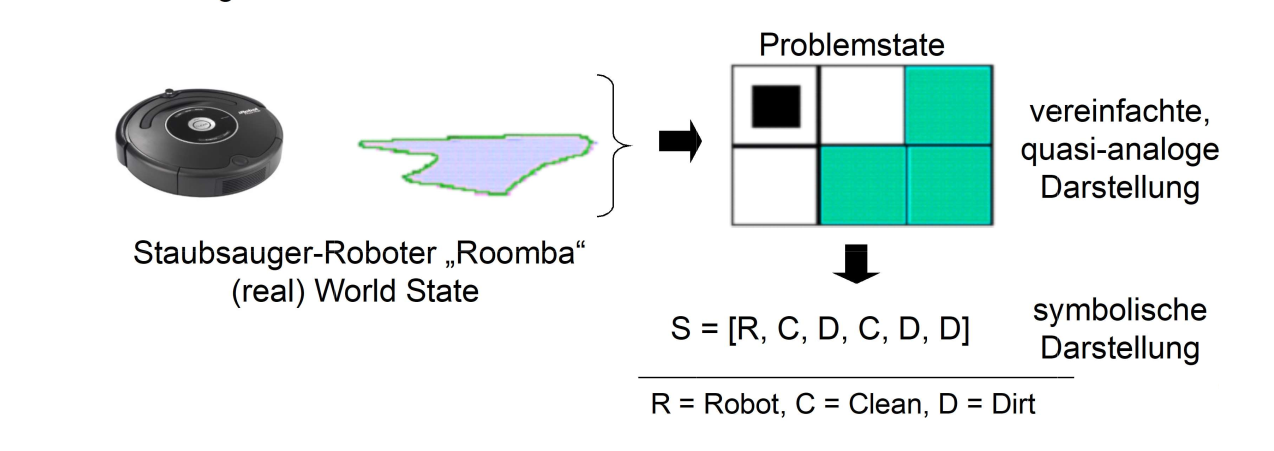
\includegraphics[width=0.8\textwidth]{figures/roomba-world-to-problem-states.png}
    \caption{Abbildung World States auf Problem States}
    \label{fig:roomba-abbildung}
\end{figure}

